\documentclass[runningheads]{llncs}
\usepackage{graphicx}
\usepackage{hyperref}
\usepackage{subcaption}
\newcommand{\lerna}{\textsc{Lerna}}
\newcommand{\z}[1]{\textsc{Z3}}
\newcommand{\mizarlarge}{\textit{M40k}}
\newcommand{\mizarsmall}{\textit{M2k}}
\begin{document}
\title{A Neural, Parallel Theorem Prover*}
\author{
	Michael Rawson*\orcidID{0000-0001-7834-1567}\inst{1} \and
	Giles Reger\inst{2}
}
\institute{
	University of Manchester, UK\\
	\email{michael@rawsons.uk}\and
	University of Manchester, UK
}
\maketitle

\begin{abstract}
	We present the \lerna{} system, a neurally-guided automatic theorem prover for first-order logic with equality.
	The system uses a neural network trained on previous proof search attempts to evaluate subgoals based directly on their structure, and hence bias proof search toward success.
	An existing first-order theorem prover is employed to dispatch easy subgoals and prune branches which cannot be solved.
	Exploration of the search space is asynchronous with respect to both the evaluation network and the existing prover, allowing for efficient batched neural network execution and for natural parallelism within the prover.
\keywords{ATP \and Graph Convolutional Network \and Tableaux \and MCTS}
\end{abstract}

\section{Background}

\subsection{First-Order Logic}
(TODO copy Giles' traditional FOL-with-equality background here)

\subsection{Automatic Theorem Provers}
(TODO copy Giles' ATP background/history here)

\subsection{Machine Learning and Theorem Proving}
(TODO talk about the intersection of ATP and ML, in particular with respect to proof search guidance)

TODO The Deep Network Guided Proof Search (DNGPS) system~\cite{DNGPS} should be mentioned, as should rlCoP~\cite{rlCoP}

\subsection{The MPTP Problem Set}
For training and evaluation purposes a set of problems exported from the Mizar Mathematical Library~\cite{mizar} by the MPTP~\cite{MPTP} system are used.
Urban et al.~\cite{rlCoP} took a subset\footnote{\url{https://github.com/JUrban/deepmath/blob/master/M2k_list}} of the large \mizarlarge{} problem set (containing 32,524 problems) and called it \mizarsmall{} (containing 2004 problems).

\section{Introduction}
Recent advances~\cite{graph-cnn,gcn,gcn-relational} in neural network systems allow for processing graph-structured data in a neural context.
Graphs are a natural representation for logical formulae as found in automatic theorem provers~\cite{formula-graph}, suggesting a new breed of \emph{neural ATP} in which proof search is guided by a neural black-box acting as ``mathematician's intuition''.
Much previous work on integrating machine-learned heuristics into automatic theorem provers has relied on hand-engineered features~\cite{MaLeCoP,FEMaLeCoP,rlCoP} or other embedding methods~\cite{ENIGMA}, which have the advantage of simplicity and relative efficiency, but do not encode all information available.
By contrast, a neural method which takes into account all information should allow for greater precision in proof guidance systems.
However, in practice there are several implementation issues which must be avoided in order for neural systems to integrate with efficient traditional ATPs.
\begin{enumerate}
	\item Proof state in such systems may be very large, such as in saturation-based provers~\cite{Vampire}, leading to training data which is impractical to learn from and slow to evaluate. The DNGPS system side-stepped this by only evaluating a single clause and the conjecture, reducing the amount of information available for the neural network in exchange for brevity.
	\item Data structures employed may be very opaque or ``unnatural'', containing artifice designed for efficiency rather than comprehension.
	\item Systems may be very sensitive to latency, which can result in the introduction of neural guidance systems crippling prover throughput and hence performance. Even with the reduced amount of data processed, DNGPS employed a two-phase approach in which the prover ran for some time with network guidance and then for the remainder without guidance.
\end{enumerate}
%
By avoiding these issues with a novel prover architecture and exploring several options to improve efficiency, the \lerna{}\footnote{\textbf{Le}arning to \textbf{R}eason with \textbf{N}eural \textbf{A}rchitectures. Lerna is also the lair of the mythical many-headed beast \textsc{Hydra}.} system explores a step toward useful neural automatic theorem provers.
\section{Design}
\label{section:Design}
\subsection{Rationale}
\subsection{Architecture}
\subsection{Implementation}

\section{Calculus}

\section{Oracle}
\label{section:oracle}
One problem with the calculus as described is that proofs can be quite lengthy, even if the goal is relatively trivial.
To rectify the situation, new goals generated by ongoing proof search are enqueued for attempted proof by an existing \emph{oracle} ATP system, as described in Section \ref{section:Design}.

\subsection{Z3}
\z3{}\cite{Z3} is an efficient and mature SMT solver, supporting a core propositional logic extended with ``theories'' such as arithmetic and datatypes.
It also notably supports first-order logic via a combination of decision procedures for decidable fragments (such as the Bernays-Sch\"onfinkel class of formulae), and heuristic quantifier instantiation routines~\cite{quantifier-instantiation}.
\z3{} is attractive for this application due to its low startup times and its ability to produce both satisfiable and unsatisfiable results.

In the \lerna{} system, we ran \z3{} as an external program (thus reducing the coupling to any particular ATP, although \z3{} has an API which might improve efficiency) with its Model-Based Quantifier Instantiation heuristic for 20 milliseconds.
This was chosen as the shortest time in which the oracle can dispatch a reasonable amount of trivial goals (and in fact \z3{} is so strong it dispatches some goals immediately: see Section \ref{section:results}).
Longer oracle runtimes might produce better performance in future, but for this experiment longer runtimes begin to conflate the performance of the oracle and the performance of the system as a whole.
This application is unusual for ATP systems --- very short runtimes, and a mix of true and false problem statements.
Running in this setting also amounts to fuzz-testing: in development of this system a bug was rediscovered in \z3{}\footnote{\url{https://github.com/Z3Prover/z3/issues/2101}} which resulted in non-termination of the prover: happily, the bug was already fixed in a newer version.

\subsection{Acting as a Preprocessor}
\lerna{} as a whole might also be seen as an intelligent pre-processor for existing ATPs in this setting: existing theorem provers are known to be sensitive to small changes in their input~\cite{clausification}, and generally make little attempt to split their input into smaller sub-goals, for parallelism~\cite{parallel} or otherwise.
The system can therefore act as an adaptor for any existing first-order ATP, adding parallelism opportunities and ``smoothing out'' sensitivity to input syntax.

\section{Learned Heuristic}
A suitable heuristic function for the system must predict a value between 0 and 1 for a given formula \(F\), where 0 represents a satisfiable goal and 1 represents unsatsfiability, based on a set of tagged formulae seen in previous proof search.
Although the data is collected by running the system itself (and therefore might be considered \emph{reinforcement} learning~\cite{reinforcement}), for this approach data collection and learning were considered separately and hence forms a classic supervised-learning problem.

\subsection{Data Collection}
A large dataset of satisfiable and unsatisfiable goals were collected by running the unguided prover on the \mizarlarge{} dataset for 10 seconds.
As soon as the prover determines the satisfiability of any sub-goal, the formula it represents and its status is recorded.
This resulted in 18,340 unsatisfiable examples and 1,845,267 satisfiable examples, occupying 6GB of disk space.
The dataset is very imbalanced (due to a combination of weakening rules producing a large number of trivially-satisfiable examples, and to prover termination after the goal is shown to be unsatisfiable), at a ratio of around 100:1.

\subsection{Translation to Graphs}
Wang et al.~\cite{formula-graph} give a translation from higher-order formulae to directed graphs, and a similar scheme is used here.
Constants, function symbols, predicate symbols, and bound variables are given their own node.
Application of functions and predicates to arguments are represented as an ``application node'' with two children: the symbol node and an ``argument list'' node representing the list of arguments.
Propositional connectives and equality have the obvious representation, while quantifiers have two children: the variable they bind and their sub-formula.

To produce an input graph from a formula \(F\), the formula is first parsed into an abstract syntax tree.
Common sub-trees up to \(\alpha\)-equivalence are merged, then the resulting directed acyclic graph has any named-symbol nodes replaced with an opaque, nameless label such as "predicate" or "variable" --- since distinct symbols remain as distinct nodes under this scheme, no information is lost other than the natural-language semantics of the symbol name.
In practice, undirected graphs improved model performance so the graph is made undirected before encoding node labels as one-hot inputs to produce the final input graphs.

An example formula's translation from
\[
	F = \forall X, \left[p\left(f(c), X\right) \wedge \lnot\left(f(c) = d\right)\right]
\]
is shown in Figure \ref{figure:translation}.

\begin{figure}
	\centering
	\begin{subfigure}{.4\textwidth}
		\centering
		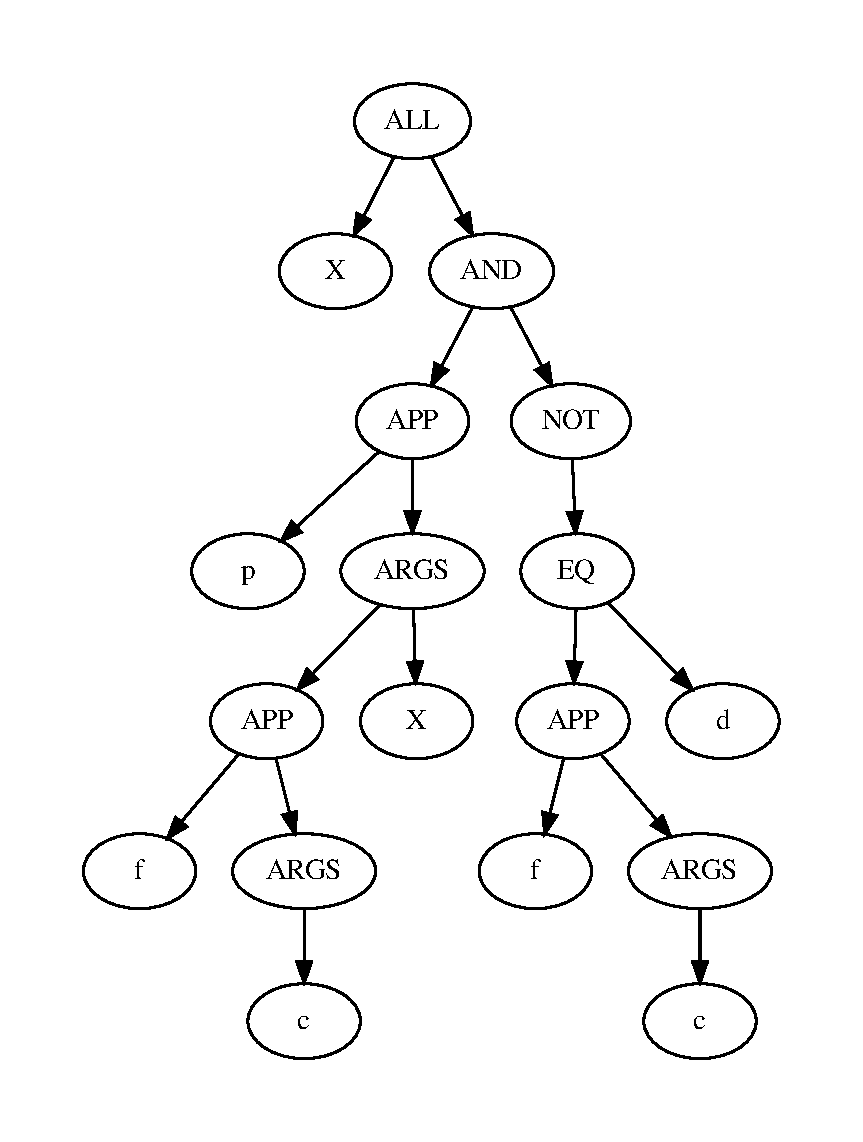
\includegraphics[width=\linewidth]{translation-ast}
		\caption{The AST for \(F\).}
	\end{subfigure}
	\begin{subfigure}{.3\textwidth}
		\centering
		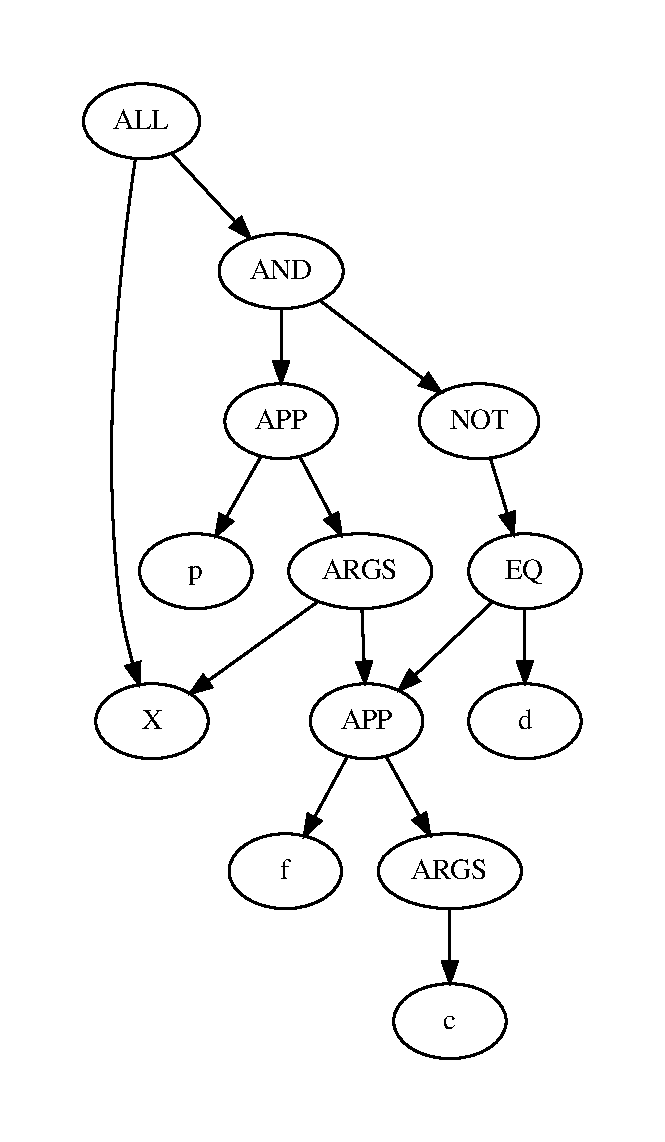
\includegraphics[width=\linewidth]{translation-graph}
		\caption{De-duplicated DAG.}
	\end{subfigure}
	\begin{subfigure}{.3\textwidth}
		\centering
		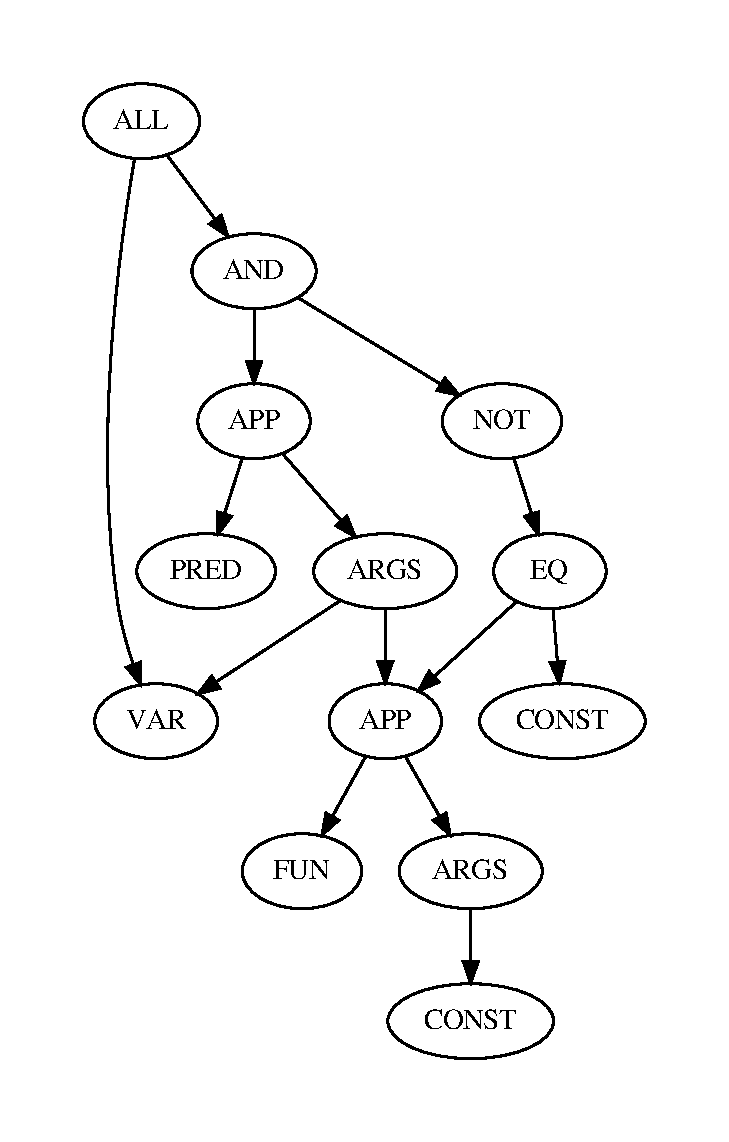
\includegraphics[width=\linewidth]{translation-nameless}
		\caption{Nameless DAG.}
	\end{subfigure}
	\begin{subfigure}{.3\textwidth}
		\centering
		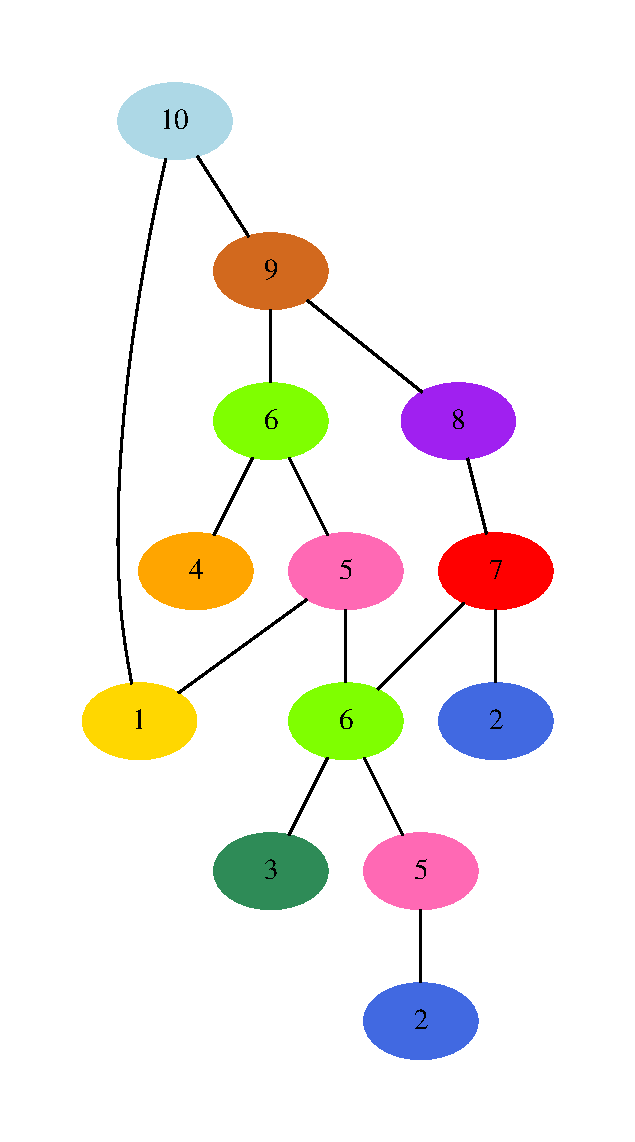
\includegraphics[width=\linewidth]{translation-undirected}
		\caption{Final result.}
	\end{subfigure}
	\caption{The translation process from \(F\) to a graph as seen by the neural network.}
	\label{figure:translation}
\end{figure}

\subsection{Augmentation}
One possible solution~\cite{imbalanced} to the problem of classification on imbalanced domains is to synthesize new data for under-represented classes --- in this case unsatisfiable formulae --- from existing data by augmenting it.
A classic example is augmenting image data by cropping, flipping or adding noise to existing images.

There are many possible ways to augment formulae graphs.
For this prototype, a simple approach is taken in which a small number of nonsense formulae are added to the graph by randomly adding nodes/edges where appropriate.
This approach has the advantage of exposing the network to ``noise'' such as additional axioms which might well occur in practice, but if the network is adequately capable of filtering these then no new formulae are actually seen.

\subsection{Neural Architecture}
TODO set fixed architecture and report on this.

\subsection{Implementation}
TODO discuss implementation with PyTorch~\cite{pytorch} and its graph-processing extension PyTorch Geometric~\cite{pytorch-geometric}.

\section{Results}
\label{section:results}
\subsection{Hardware}
All results collected on commodity hardware (TODO talk about specs).

\subsection{Benchmark Results}

Table \ref{table:m2k-results} shows the total number of theorems proved using various configurations of \z3 and LeRNA on the M2k dataset.
\z3 ran for a full 10 seconds to establish baseline performance, then as an oracle for 20 milliseconds to determine the number of ``trivial'' problems.
LeRNA ran on an identical dataset, first without guidance from the neural heuristic, then with guidance.

\begin{table}
	\caption{Total theorems proved on the M2k dataset.}
	\centering
	\begin{tabular}{r | c}
		\textbf{Configuration} & \textbf{Theorems Proved}\\
		\hline
		\z3 (10s, as baseline) & 1216\\
		\z3 (20ms, as oracle) & 711\\
		LeRNA, unguided (10s, with oracle) & 969\\
		LeRNA, guided (10s, with oracle) & 1012\\
						      & FIXME there is a bug, these ought be better\\
	\end{tabular}
	\label{table:m2k-results}
\end{table}

\section{Conclusions}
\section{Future Work}
The style of theorem prover described opens many new directions for future work and improvements to the system.
As \lerna{} is a very new system, there is likely much to be gained by simple engineering and tuning: for example, the UCT exploration parameter \(c\) has been left at its theoretical optimum value \(\sqrt{2}\), but it is likely that a higher value will account for neural network inaccuracies and hence improve performance.
Training on, benchmarking with, and optimising for other datasets (such as the famous TPTP benchmark~\cite{TPTP}) is also left as future work.

\subsection{Proof Search}
\lerna{} is well-suited for long-term proof search attempts in mathematics, such as those employed in the AIM project~\cite{AIM}: search is stable over time and does not produce a combinatorial explosion in the same way that some traditional systems tend to after a short period.
Additionally, the amount of information (``confidence'') in the system grows over time, as a result of a growing number of oracle invocations and neural network evaluations.
Proof search can in principle be manually inspected more easily than in saturation-based provers to examine promising subgoals and remove known falsehoods from the search space.
The authors hope to explore applying the system to this interesting domain.

Another future direction for proof search is a principled incomplete mode, in which branches deemed sufficiently uninteresting by the heuristic are pruned, perhaps in response to time or memory constraints as seen in limited resource strategies~\cite{LRS}.
This approach, while clearly incomplete, would significantly accelerate proof search in the direction of more promising search within the available resources.

\subsection{Prover Calculus}
The calculus currently employed is deliberately na\"ive, so much work is planned here.
In particular, the simplification routines can be improved to remove more trivial sub-formulae.
While in general the oracles' pre-processing will remove these, they serve as noise for the neural network and might also increase the number of inference steps required to reach a proof.

As one possible view of this approach is as an intelligent pre-processor (as mentioned in Section \ref{section:oracle}) for an existing efficient ATP, a greater number of aggressive and/or weakening inferences might be included in the calculus.
For instance, \emph{prenexing} (or conversely \emph{miniscoping}) formulae can have a significant effect on proof search~\cite{clausification} for some theorem provers, so including suitable quantifier-manipulation rules might prove to be a useful extension.

Generalising further, ideas from other refutation-tableaux calculi could well be suitable for this system.
In particular, the authors are attempting to integrate an adapted connection rule from the non-clausal connection calculus~\cite{non-clausal-connections}, as used in nanoCoP~\cite{nanocop}, in order to reduce the number of proof steps required to instantiate universal quantifiers.

Finally, this prover architecture can support other logics without excessive modification.
Given that \z3 is already capable of supporting many \emph{theories}, such as arithmetic or datatypes, a many-sorted first order logic such as those described by SMTLIB~\cite{smtlib} or the TFF0 dialect of TPTP~\cite{tff0} seems an appropriate first step.

\subsection{Oracle}
While \z3 is a strong theorem prover in its own right and performs well here, it remains to be seen if it is the best for this application.
Other ATPs (or indeed counter-example-finding systems) should be tested as it involves minimal engineering effort.
A \emph{portfolio} of several oracle systems working in tandem might also be considered, although of course this will eventually retard proof search linearly in the number of systems present.

Reducing the number of oracle invocations is another area for optimisation.
Currently, the system calls an oracle for every new subgoal generated.
It seems unlikely that the subgoal is materially easier to dispatch than its parent (especially in the case of propositional inferences that do not split the goal), so heuristically or probabilistically removing such subgoals from the oracle's queue is a possible area for improvement.

\lerna{} does not currently use any information from the oracle beyond its status: using auxiliary information such as satisfying models or unused formulae could well aid proof search.

\subsection{Machine-Learned Heuristic}
Many other graph-based neural architectures are possible.
PyTorch Geometric alone currently includes nearly 40 other graph-specific neural layers pre-programmed from the literature.
Neural models specifically for theorem proving are relatively under-studied.
To combat this, data used for this paper will be published in the near future so that the machine-learning community can improve upon our simple models.

Different approaches to formula-to-graph translation, symbol embeddings, data augmentation, and model integration may also be explored.

\section{Acknowledgements}
The authors wish to thank Josef Urban and his group in \v{C}VUT, Prague for their help and encouragement with early iterations of this work and for supplying the Mizar dataset used in this paper.

\bibliographystyle{splncs04}
\bibliography{references}
\end{document}
